\documentclass{article}
% Preprint: non-anonymous, footer ``Preprint.'', no submission line numbers.
\usepackage[preprint]{neurips_2026}

\usepackage[utf8]{inputenc}
\usepackage[T1]{fontenc}
\usepackage{url}
\usepackage{booktabs}
\usepackage{amsmath}
\usepackage{amsfonts}
\usepackage{nicefrac}
\usepackage{microtype}
\usepackage{xcolor}
\usepackage{graphicx}
% Load hyperref last (avoids option clashes; PDF bookmarks for sections).
\usepackage[hidelinks]{hyperref}

\title{Adversarial Robustness on STL-10: A Comparative Study of Clean, FGSM, PGD, and TRADES Training}

\author{%
  Ashfak Yeafi \\
  Department of Biosystems and Agricultural Engineering \\
  Michigan State University \\
  \texttt{yeafiash@msu.edu}%
}

\begin{document}

\maketitle

\begin{abstract}
Adversarial examples can fool deep classifiers with small, often human-imperceptible perturbations. This report studies robustness on STL-10 using ResNet-18 under four training regimes: standard empirical risk minimization, FGSM adversarial training, PGD adversarial training, and TRADES. All models are evaluated under clean accuracy and white-box FGSM and PGD attacks at multiple $\ell_\infty$ budgets. The experiments exhibit the expected robustness--accuracy tradeoff: the clean-trained model reaches 72.5\% clean accuracy but only 0.12\% accuracy under PGD at $\epsilon=8/255$, whereas robust training raises strong-PGD accuracy to 31.7--33.4\% at the cost of lower clean accuracy. Beyond aggregate curves, the study reports attack transfer matrices, per-class PGD robustness, resolution-shift evaluation, and qualitative attack visualizations. Code, result tables, and figures are publicly available at \url{https://github.com/AshfakYeafi/CSE-850}.
\end{abstract}

\section{Introduction}
Deep neural networks for image classification remain vulnerable to adversarial perturbations: small changes to the input can induce large changes in the predicted label while leaving the image visually plausible to humans. Quantifying this failure mode and comparing training-time defenses is a core theme in adversarial machine learning. This report presents an empirical study on STL-10 using a single codebase that trains and evaluates ResNet-18 under (i) clean training, (ii) FGSM adversarial training, (iii) PGD adversarial training, and (iv) TRADES.

The objectives are to:
\begin{itemize}
\item characterize the clean-versus-robust accuracy tradeoff across training methods;
\item compare FGSM and PGD white-box attacks at several $\ell_\infty$ radii;
\item analyze transfer attacks, per-class robustness, and sensitivity to input resolution; and
\item relate quantitative metrics to qualitative attack visualizations.
\end{itemize}

\subsection{Intellectual merits}
Individual project; merits claimed are:
\begin{itemize}
\item \textbf{Controlled comparison:} Four training strategies share data handling, optimization defaults, and evaluation code.
\item \textbf{Multi-baseline evaluation:} Clean accuracy plus FGSM and PGD at $\epsilon\in\{2/255,4/255,8/255\}$.
\item \textbf{Extra analyses:} Transfer matrices, per-class robustness, resolution shift, and attack images alongside tables.
\item \textbf{Honest limitation:} TRADES did not beat PGD training here at the strongest PGD budget without extra tuning of $\beta$ and schedule.
\end{itemize}

\subsection{Problem formulation}
Let $f_\theta:\mathcal{X}\rightarrow\mathbb{R}^K$ be a classifier with parameters $\theta$, input $x$, and label $y$. Standard empirical risk minimization (ERM) solves:
\[
\min_\theta \; \mathbb{E}_{(x,y)\sim\mathcal{D}} \left[\ell\!\left(f_\theta(x),y\right)\right].
\]
Under adversarial evaluation, an attacker perturbs inputs inside an $\ell_\infty$ ball:
\[
\mathcal{B}_\epsilon(x)=\{x' : \|x'-x\|_\infty \le \epsilon\},
\]
and seeks to maximize loss. Robust optimization can be written as
\[
\min_\theta \; \mathbb{E}_{(x,y)\sim\mathcal{D}}\left[\max_{x'\in\mathcal{B}_\epsilon(x)} \ell\!\left(f_\theta(x'),y\right)\right].
\]
FGSM and PGD provide practical approximations to the inner maximization, while TRADES replaces this objective with an explicit clean/robust tradeoff term.

\section{Method}
\subsection{Training setups}
All models use a ResNet-18 backbone trained on STL-10. We evaluate the following:
\begin{itemize}
\item \textbf{Clean Model}: standard empirical risk minimization.
\item \textbf{FGSM Adversarial Model}: adversarial training with FGSM samples.
\item \textbf{PGD Adversarial Model}: adversarial training with multi-step PGD.
\item \textbf{TRADES Model}: robust optimization with objective
\[
\mathcal{L}_{\text{TRADES}} = \mathcal{L}_{\text{CE}}(f(x),y) + \beta \cdot \mathrm{KL}\left(f(x+\delta)\,\|\,f(x)\right),
\]
where this run uses $\beta=6$, $\epsilon=8/255$, $\alpha=2/255$, and 10 inner steps.
\end{itemize}

\subsection{Attack definitions}
Given loss $\ell(f_\theta(x),y)$, FGSM computes a one-step perturbation:
\[
x^{\text{adv}} = \Pi_{\mathcal{B}_\epsilon(x)}\!\left(x + \epsilon \cdot \mathrm{sign}\!\left(\nabla_x \ell(f_\theta(x),y)\right)\right),
\]
where $\Pi$ is projection onto valid pixel range and perturbation set.

PGD performs iterative ascent:
\[
x_{t+1}^{\text{adv}} = \Pi_{\mathcal{B}_\epsilon(x)}\!\left(x_t^{\text{adv}} + \alpha \cdot \mathrm{sign}\!\left(\nabla_x \ell(f_\theta(x_t^{\text{adv}}),y)\right)\right),
\]
starting from random or clean initialization and repeating for $T$ steps.

\subsection{Threat model and protocol}
The evaluation uses an untargeted white-box threat model with full gradient access at test time. Perturbations lie in $\ell_\infty$ balls of radius $\epsilon\in\{2/255,4/255,8/255\}$. This is a standard first-order benchmark; stronger adaptive evaluations could be added in future work. All models share the same data splits and preprocessing so that reported differences are attributable to training and evaluation choices, not implementation drift.

\subsection{Evaluation protocol}
Each model is evaluated on:
\begin{itemize}
\item \textbf{Clean accuracy}
\item \textbf{FGSM attacks}: $\epsilon \in \{2/255,4/255,8/255\}$
\item \textbf{PGD attacks}: $\epsilon \in \{2/255,4/255,8/255\}$
\end{itemize}
We additionally report transfer attacks, per-class PGD robustness at strongest epsilon, and robustness under resolution shift (96 to 48 pixels).

\subsection{Reproducibility details}
Experiments use fixed random seeds and consistent logging. Each run writes CSV outputs for main evaluation, transfer attacks, per-class robustness, resolution analysis, and TRADES training dynamics. Figures are regenerated from the CSV outputs using \texttt{main.py} (including \texttt{report\_viz}) so numbers and plots stay aligned.

\section{Main results}
\subsection{Overall robustness comparison}
Table~\ref{tab:main-acc} summarizes key results.

\begin{table}[t]
\centering
\caption{Clean and adversarial accuracy (\%) on STL-10. Strong attack corresponds to $\epsilon=8/255$.}
\label{tab:main-acc}
\begin{tabular}{lccc}
\toprule
\textbf{Model} & \textbf{Clean} & \textbf{FGSM @8/255} & \textbf{PGD @8/255} \\
\midrule
Clean Model & 72.50 & 3.23 & 0.12 \\
FGSM Adversarial Model & 61.49 & 34.75 & 31.84 \\
PGD Adversarial Model & 57.88 & 35.38 & 33.39 \\
TRADES Model & 54.55 & 32.90 & 31.74 \\
\bottomrule
\end{tabular}
\end{table}

The clean model provides the highest nominal performance but almost no robustness under strong PGD. Robust training methods substantially improve adversarial accuracy. In this experiment, PGD adversarial training is best under strongest PGD attack.

\begin{figure}[t]
\centering
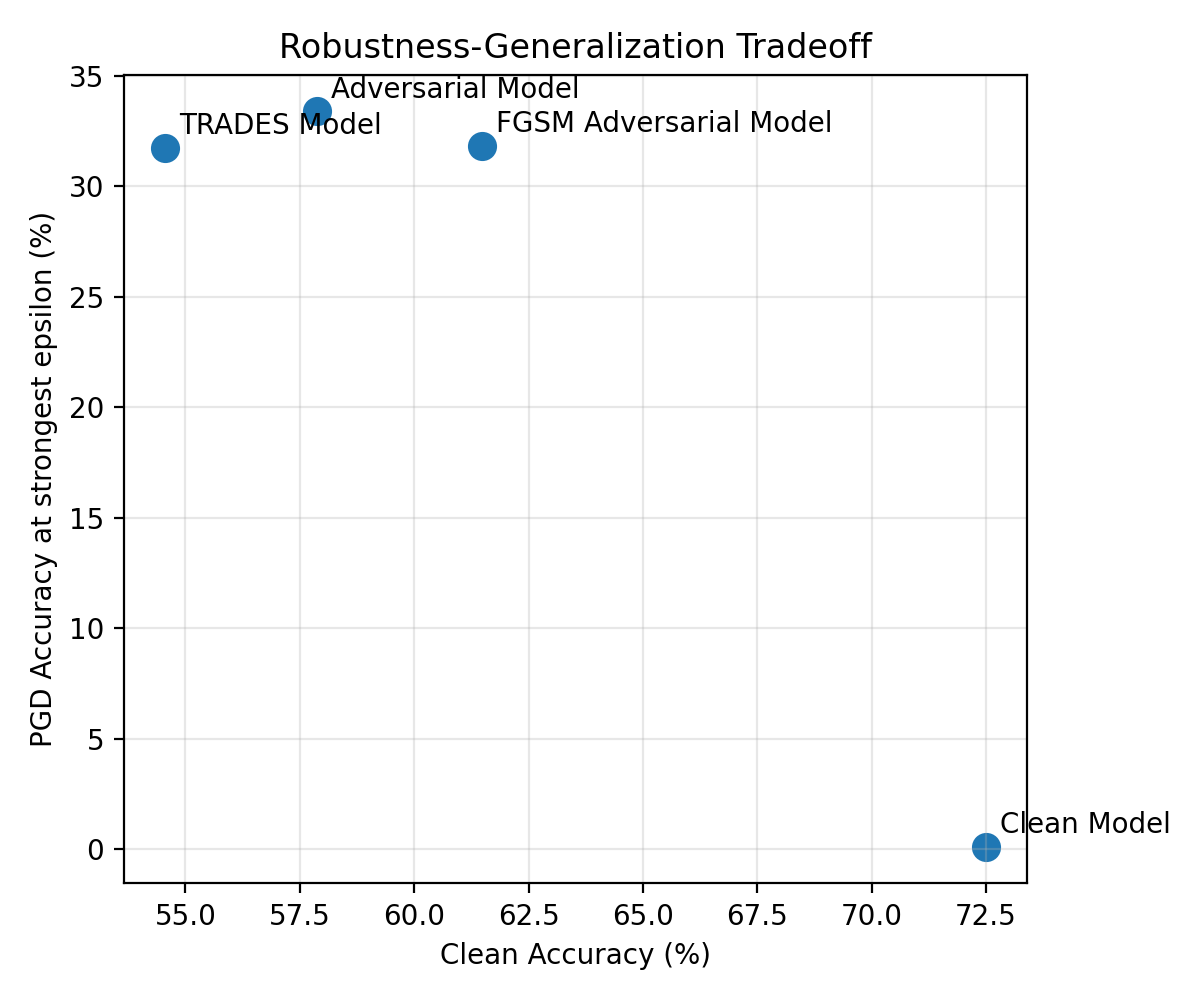
\includegraphics[width=0.8\linewidth]{../outputs/plots/report/clean_vs_robust_tradeoff_stl10.png}
\caption{Robustness-generalization tradeoff. Models with higher adversarial accuracy at strong PGD generally sacrifice clean accuracy.}
\label{fig:tradeoff}
\end{figure}

\subsection{TRADES training dynamics}
TRADES loss decreases from 2.56 to 1.39 over 50 epochs. Clean test accuracy increases from 27.45\% to 54.55\%, with peak 56.20\% near epoch 48.

\begin{figure}[t]
\centering
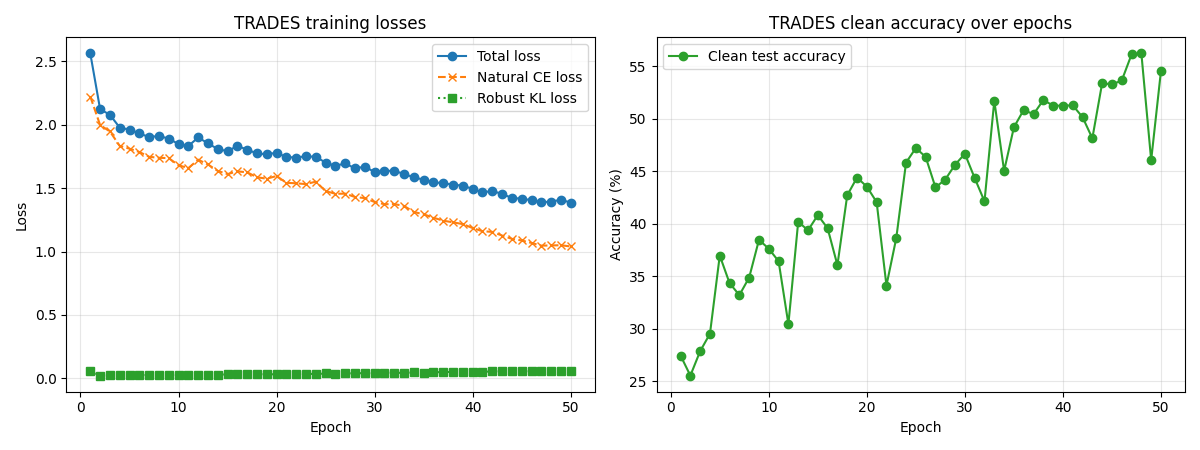
\includegraphics[width=\linewidth]{../outputs/plots/trades_training_curves_stl10.png}
\caption{TRADES training curves from logged CSV: total loss, natural loss, robust loss, and clean test accuracy by epoch.}
\label{fig:trades-curves}
\end{figure}

\subsection{Ablation on PGD training steps}
\begin{table}[t]
\centering
\caption{Ablation over PGD adversarial training steps.}
\label{tab:ablation}
\begin{tabular}{lcc}
\toprule
\textbf{PGD steps} & \textbf{Clean acc (\%)} & \textbf{PGD acc @8/255 (\%)} \\
\midrule
3 & 66.04 & 32.31 \\
7 & 56.68 & 36.56 \\
10 & 56.15 & 36.29 \\
\bottomrule
\end{tabular}
\end{table}

Increasing PGD steps improves robustness from 3 to 7 steps but reduces clean accuracy, with diminishing robustness gains beyond 7 steps.

\subsection{Quantitative interpretation}
The strongest tested setting (PGD at $\epsilon=8/255$) summarizes behavior at the largest budget in the table. Relative to the clean model's 0.12\% accuracy under that attack, PGD adversarial training gains about $33.27$ percentage points (33.39\% vs.\ 0.12\%); FGSM adversarial training and TRADES gain about $31.72$ and $31.62$ points (31.84\% and 31.74\% vs.\ 0.12\%), respectively. Thus robust training yields large relative improvements even though absolute robust accuracies remain moderate on STL-10 at this scale.

\section{Extended analysis}
\subsection{Transfer attacks}
\begin{figure}[t]
\centering
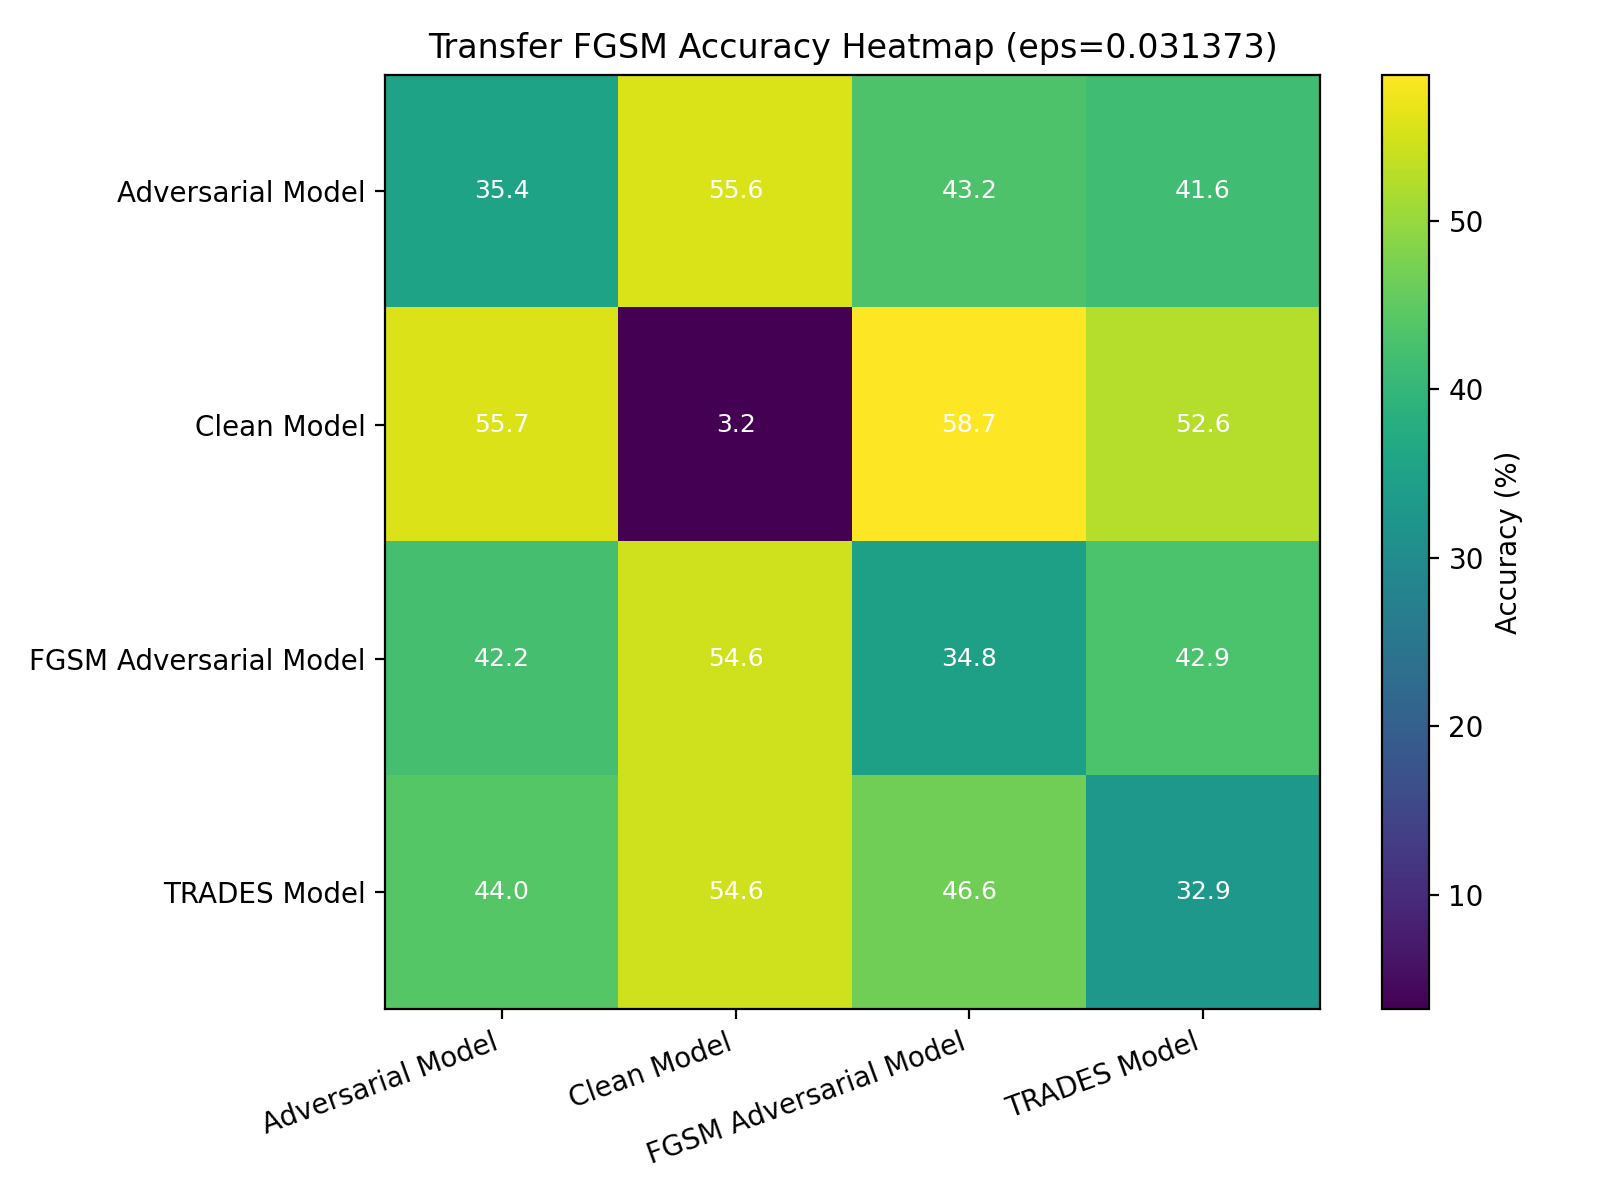
\includegraphics[width=0.48\linewidth]{../outputs/plots/report/transfer_heatmap_fgsm_stl10.png}
\hfill
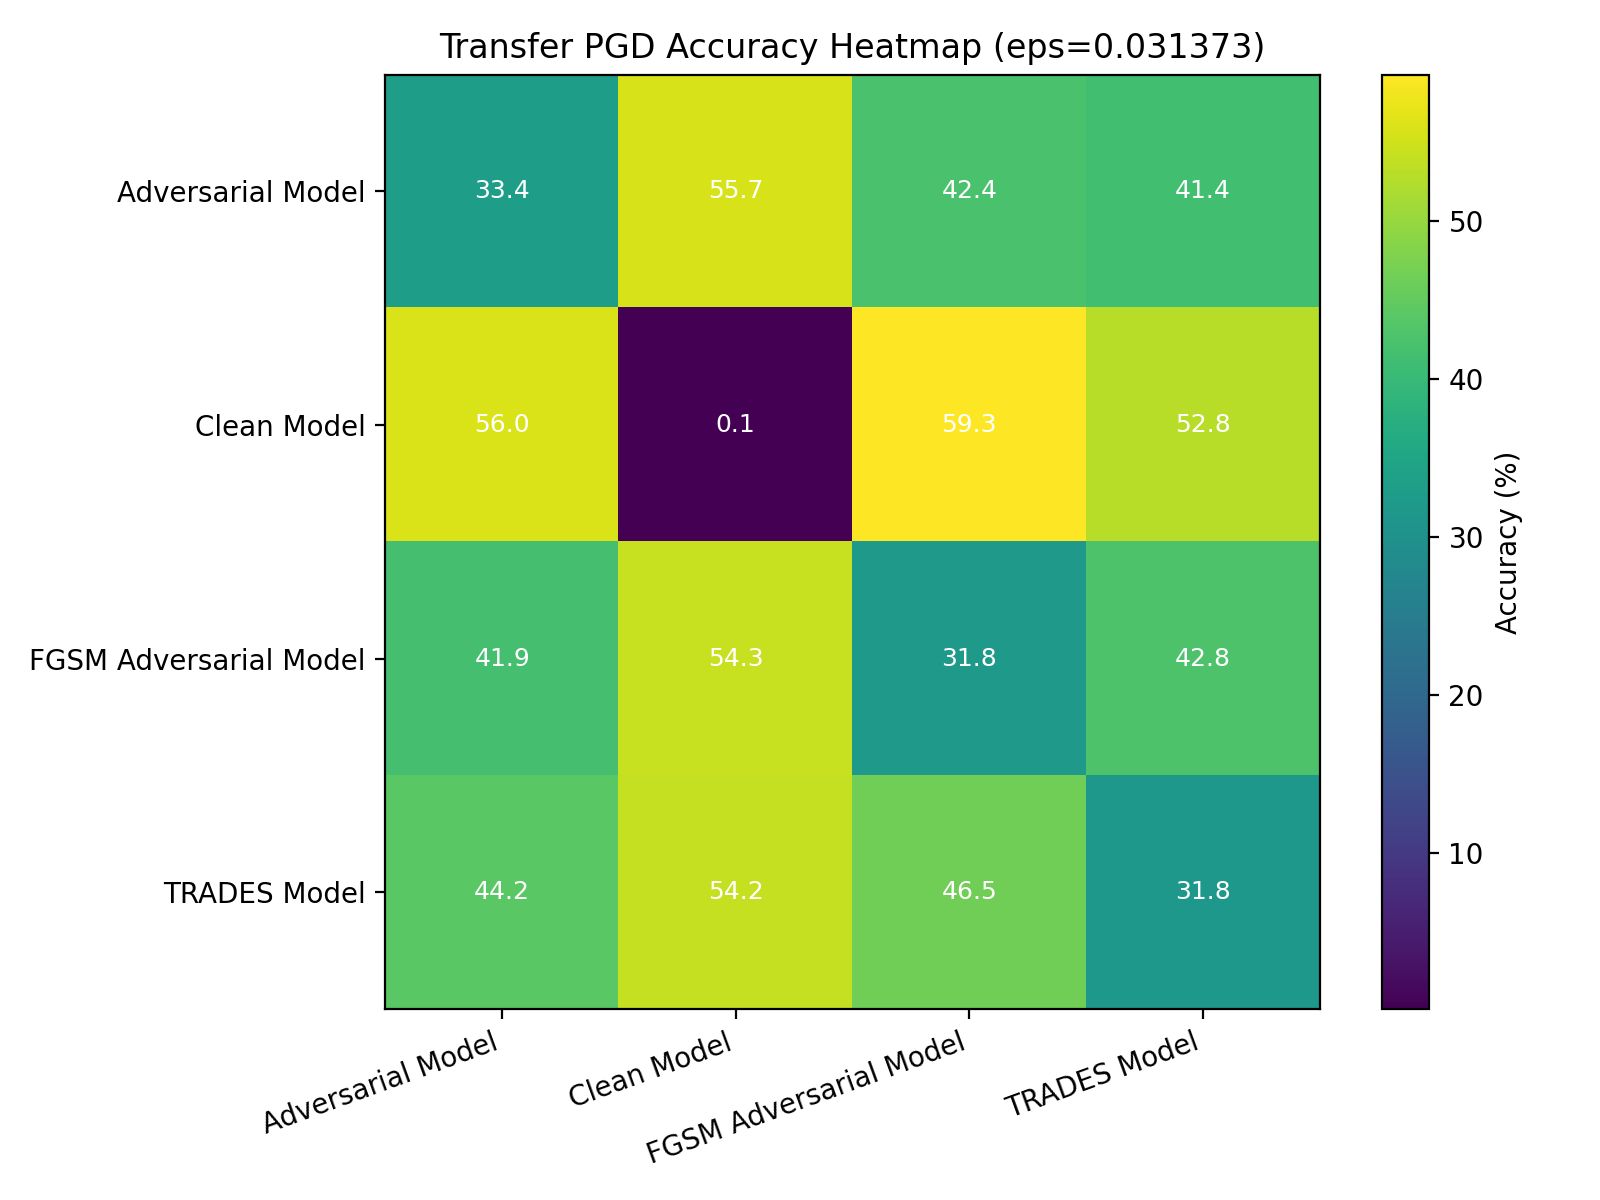
\includegraphics[width=0.48\linewidth]{../outputs/plots/report/transfer_heatmap_pgd_stl10.png}
\caption{Transfer attack heatmaps at strongest epsilon. Rows: source model used to generate adversarial examples. Columns: target model used for prediction.}
\label{fig:transfer}
\end{figure}

Transfer results show clear asymmetry: attacks crafted on the clean model transfer less effectively to robust models than to itself, while attacks crafted on robust models can still degrade clean targets due to decision boundary mismatch.

To summarize transfer behavior formally, let $A_{s\rightarrow t}(\epsilon)$ denote target-model accuracy when adversarial examples are generated on source model $s$ and evaluated on target model $t$. We report transfer matrices over $(s,t)$ pairs and compare diagonal terms ($s=t$, white-box) to off-diagonal terms ($s\neq t$, transfer). The observed diagonal-off-diagonal gap supports the expectation that transfer attacks are often weaker than direct white-box attacks, though still informative.

\subsection{Per-class robustness}
\begin{figure}[t]
\centering
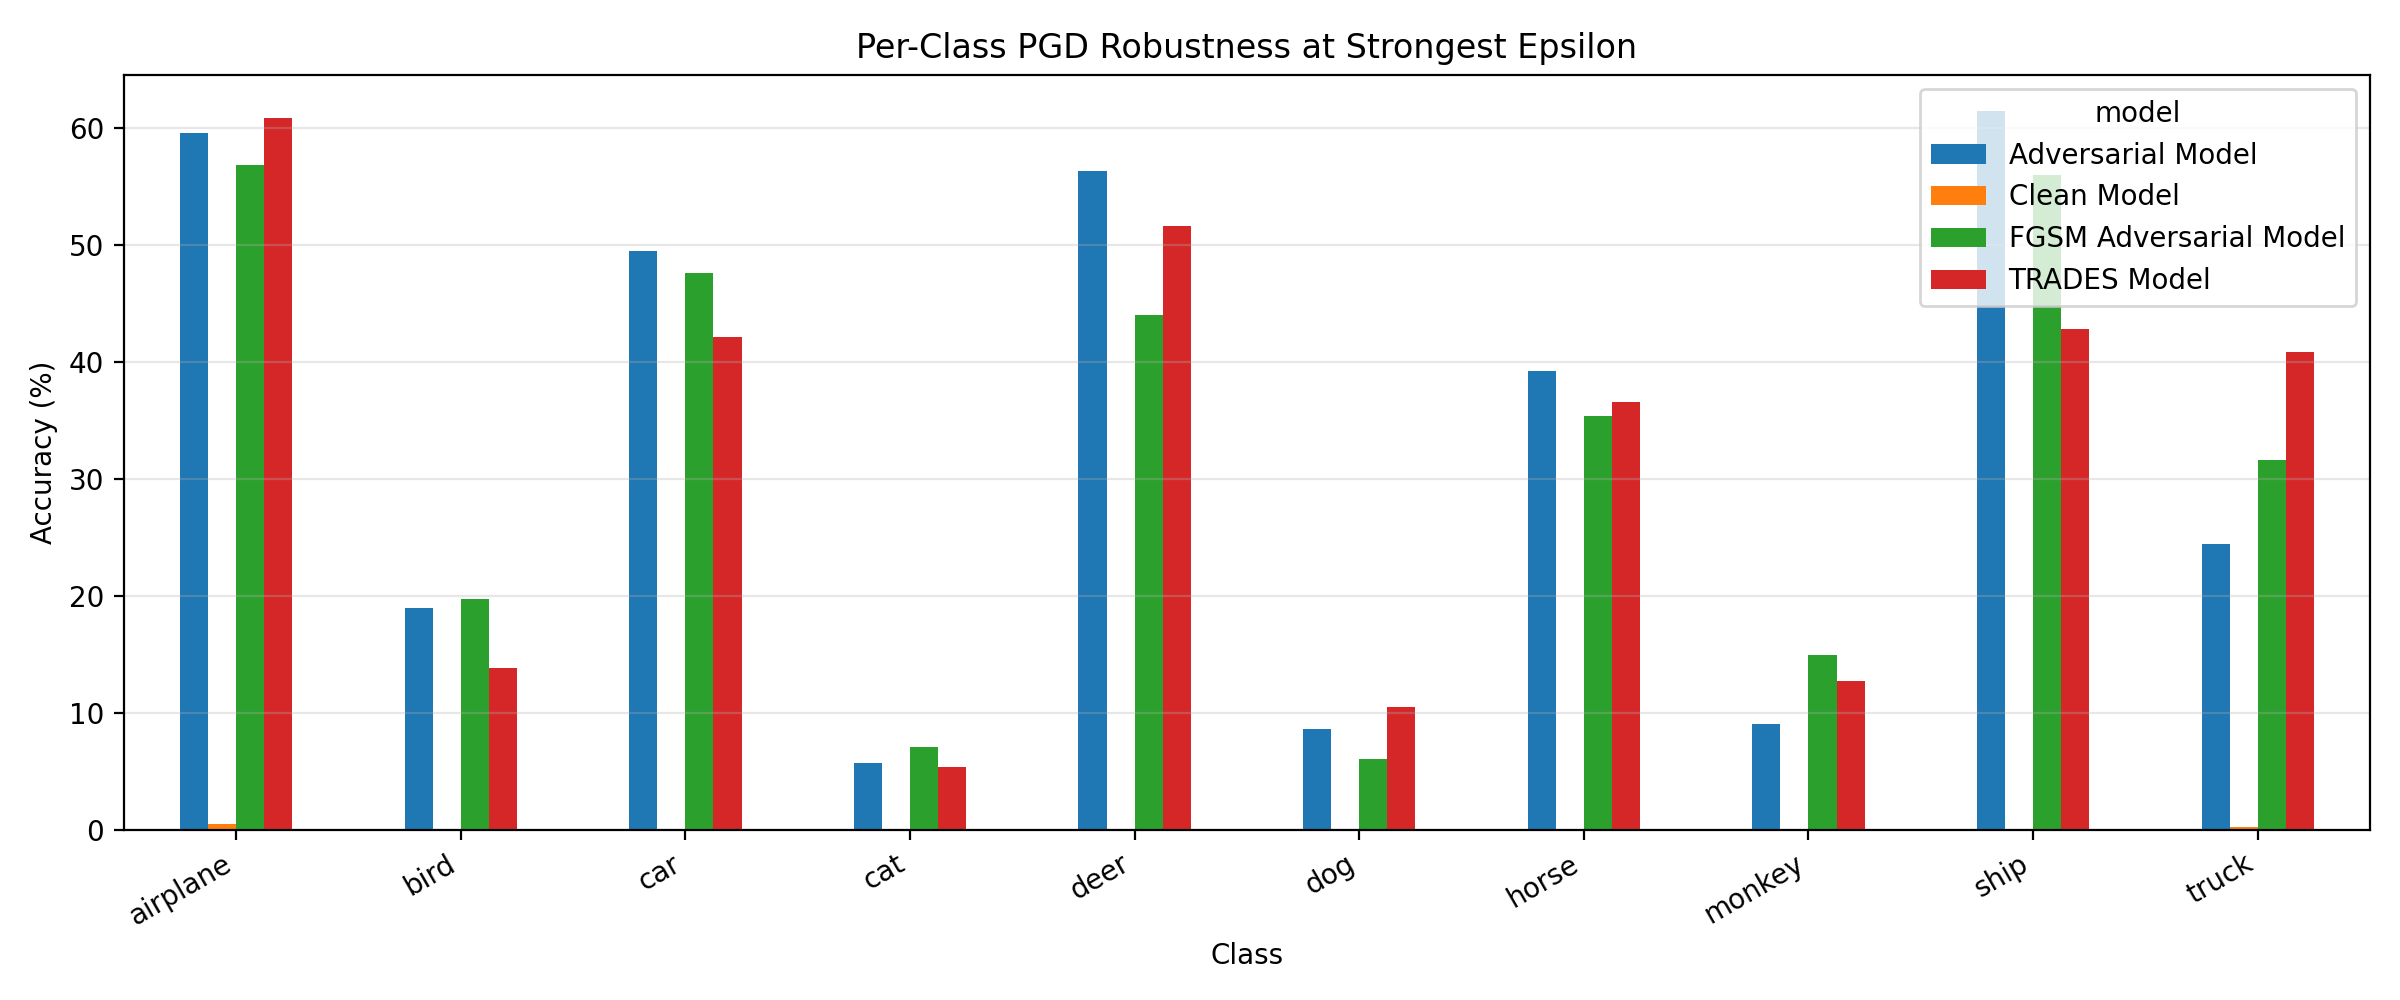
\includegraphics[width=\linewidth]{../outputs/plots/report/per_class_grouped_pgd_stl10.png}
\caption{Per-class PGD robustness at strongest epsilon. Robust models show substantial class-wise variation.}
\label{fig:perclass}
\end{figure}

Class-wise robustness is non-uniform. For robust models, classes like airplane and ship remain relatively stable, while cat/dog/monkey are consistently harder.

\subsection{Attack example visualizations}
Each panel shows clean input, adversarial image, and perturbation map for the listed attack.

\begin{figure}[t]
\centering
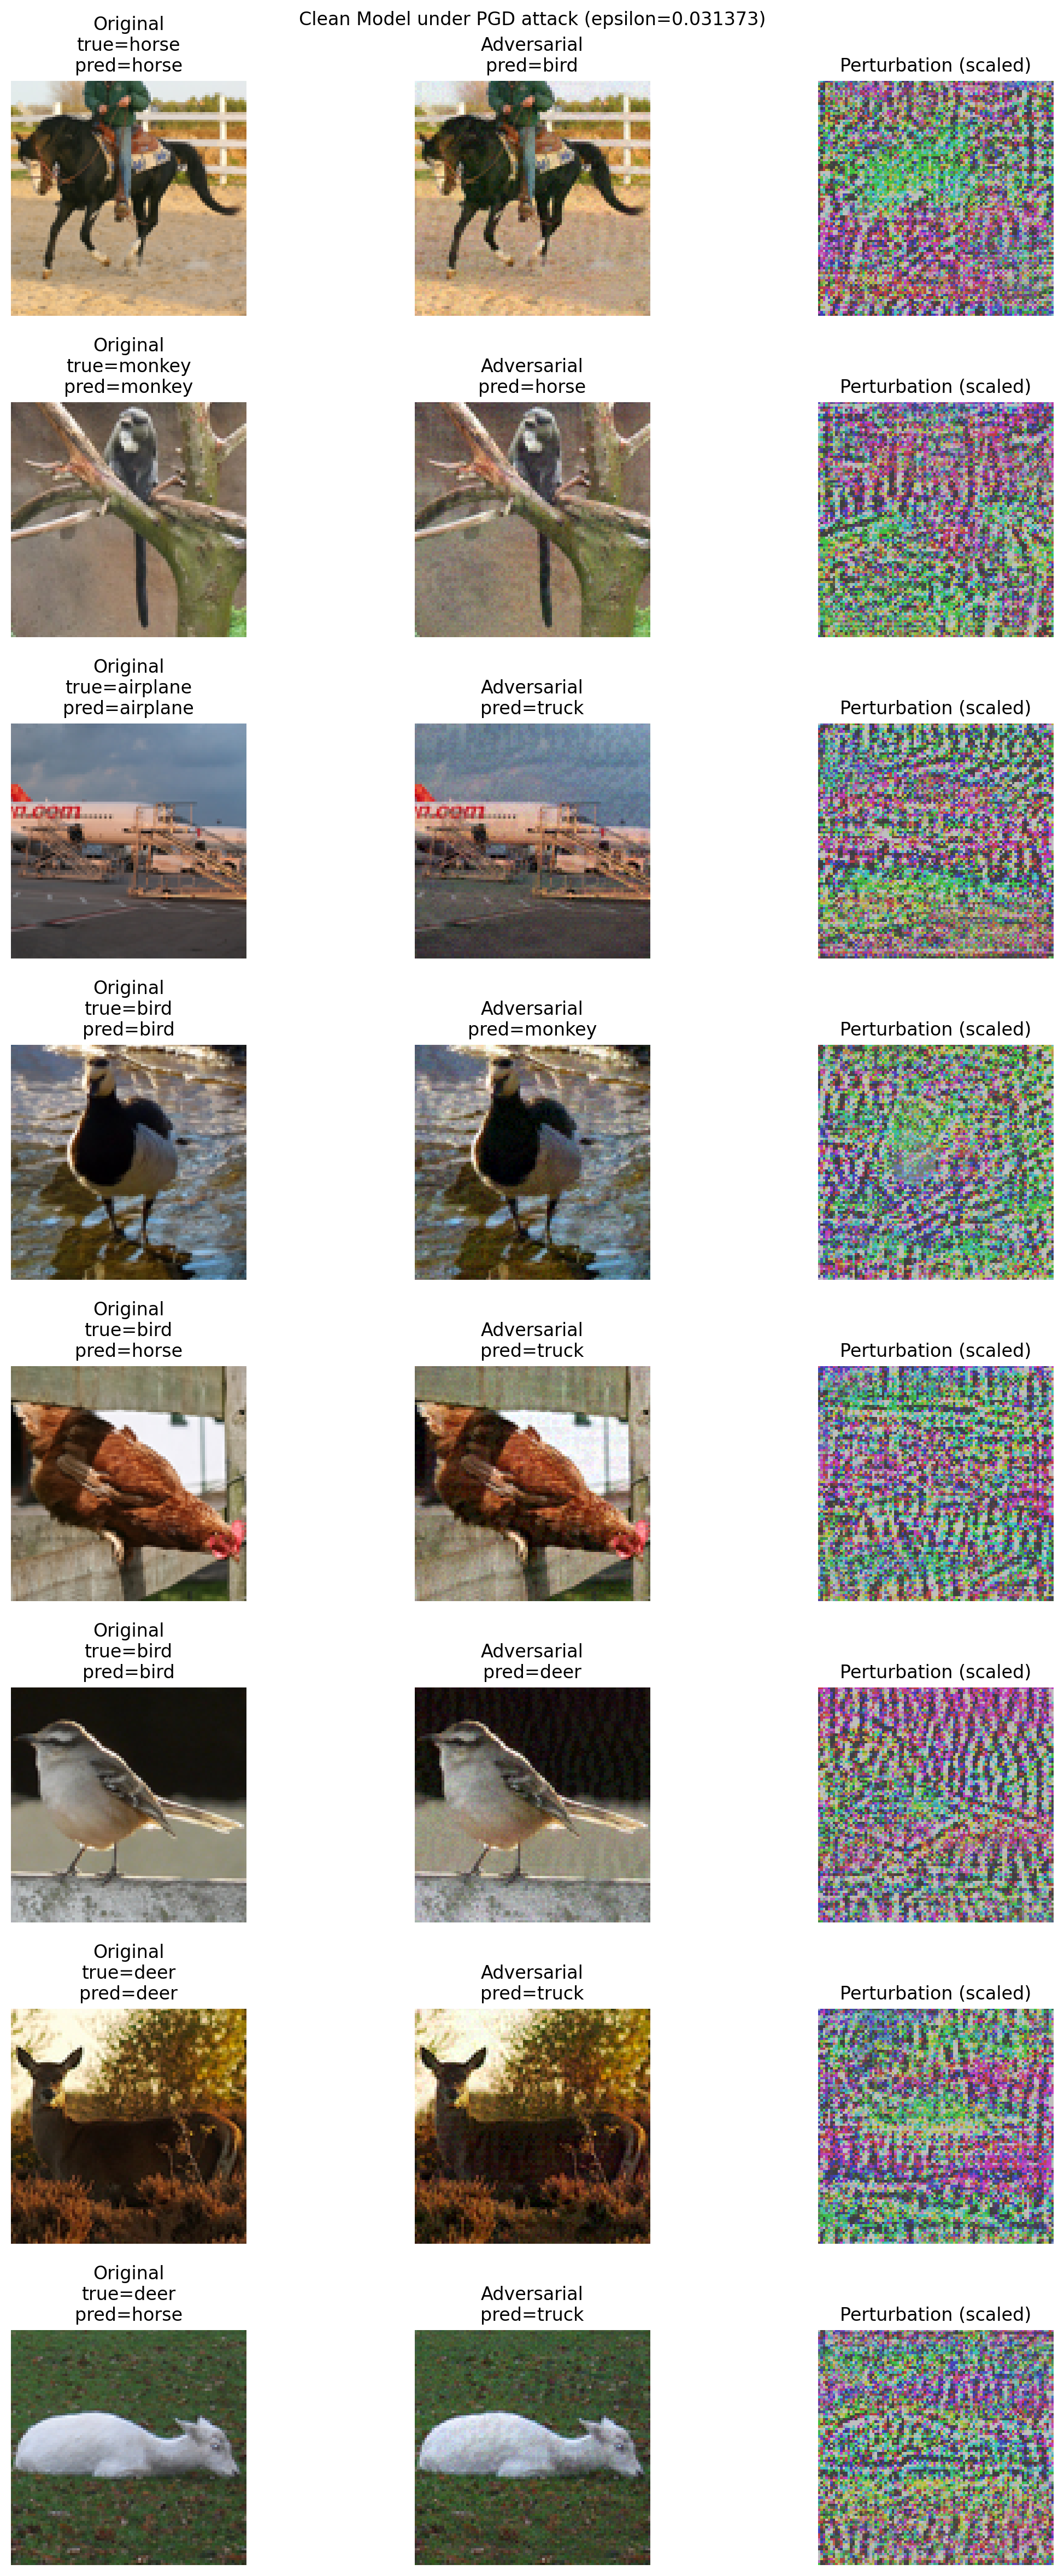
\includegraphics[width=0.49\linewidth]{../outputs/plots/attack_examples/clean_pgd_eps_0.031373.png}
\hfill
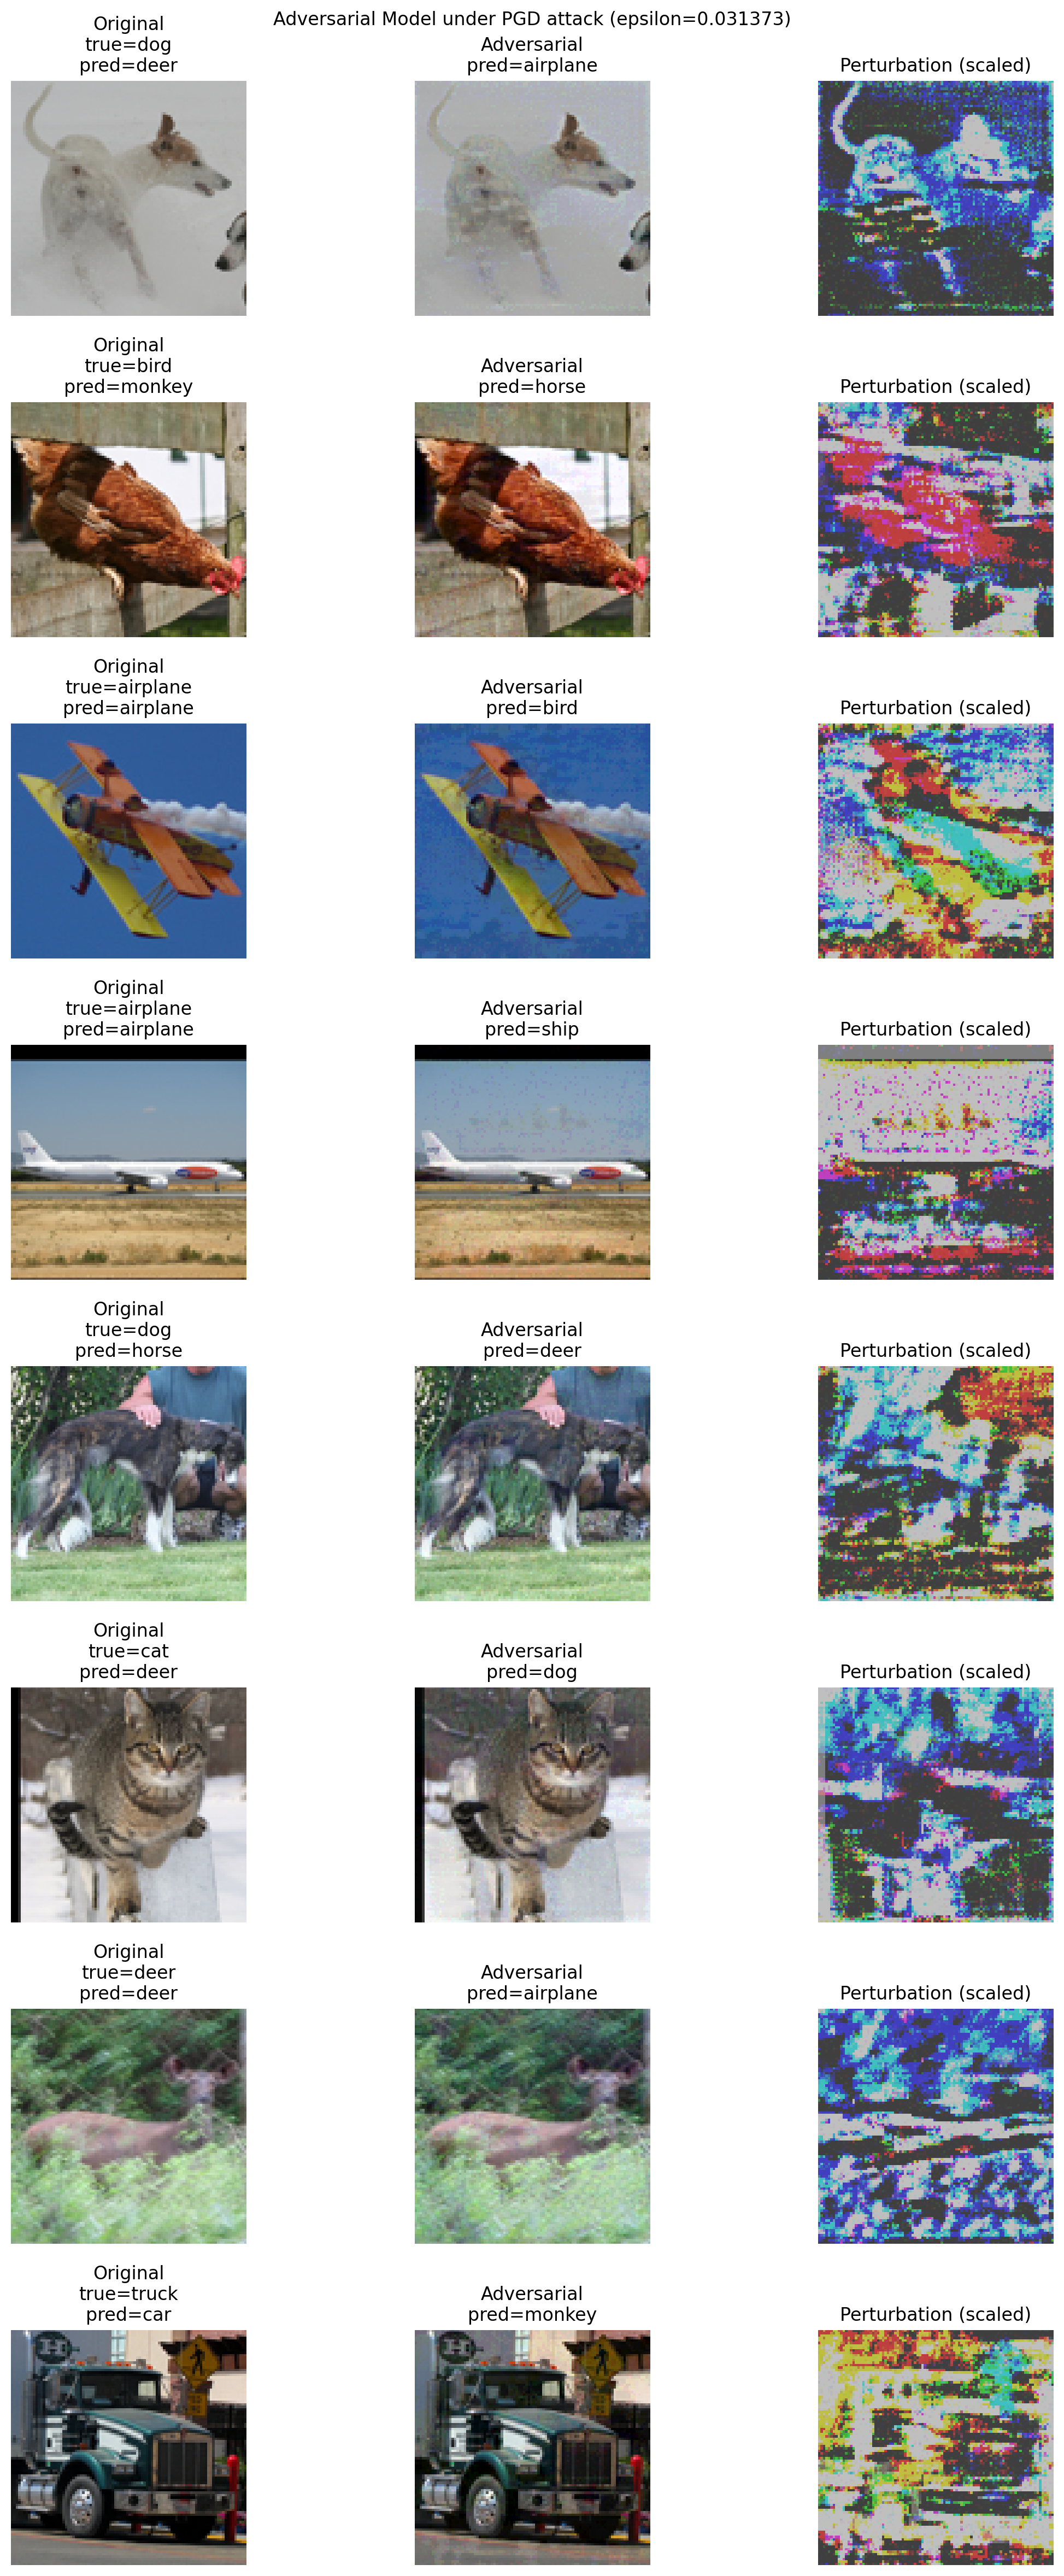
\includegraphics[width=0.49\linewidth]{../outputs/plots/attack_examples/adv_pgd_eps_0.031373.png}
\caption{PGD at $\epsilon=8/255$: clean-trained model (left) versus PGD-trained model (right). Perturbations are small but change predictions more easily on the clean-trained network.}
\label{fig:attack-viz-clean-adv}
\end{figure}

\begin{figure}[t]
\centering
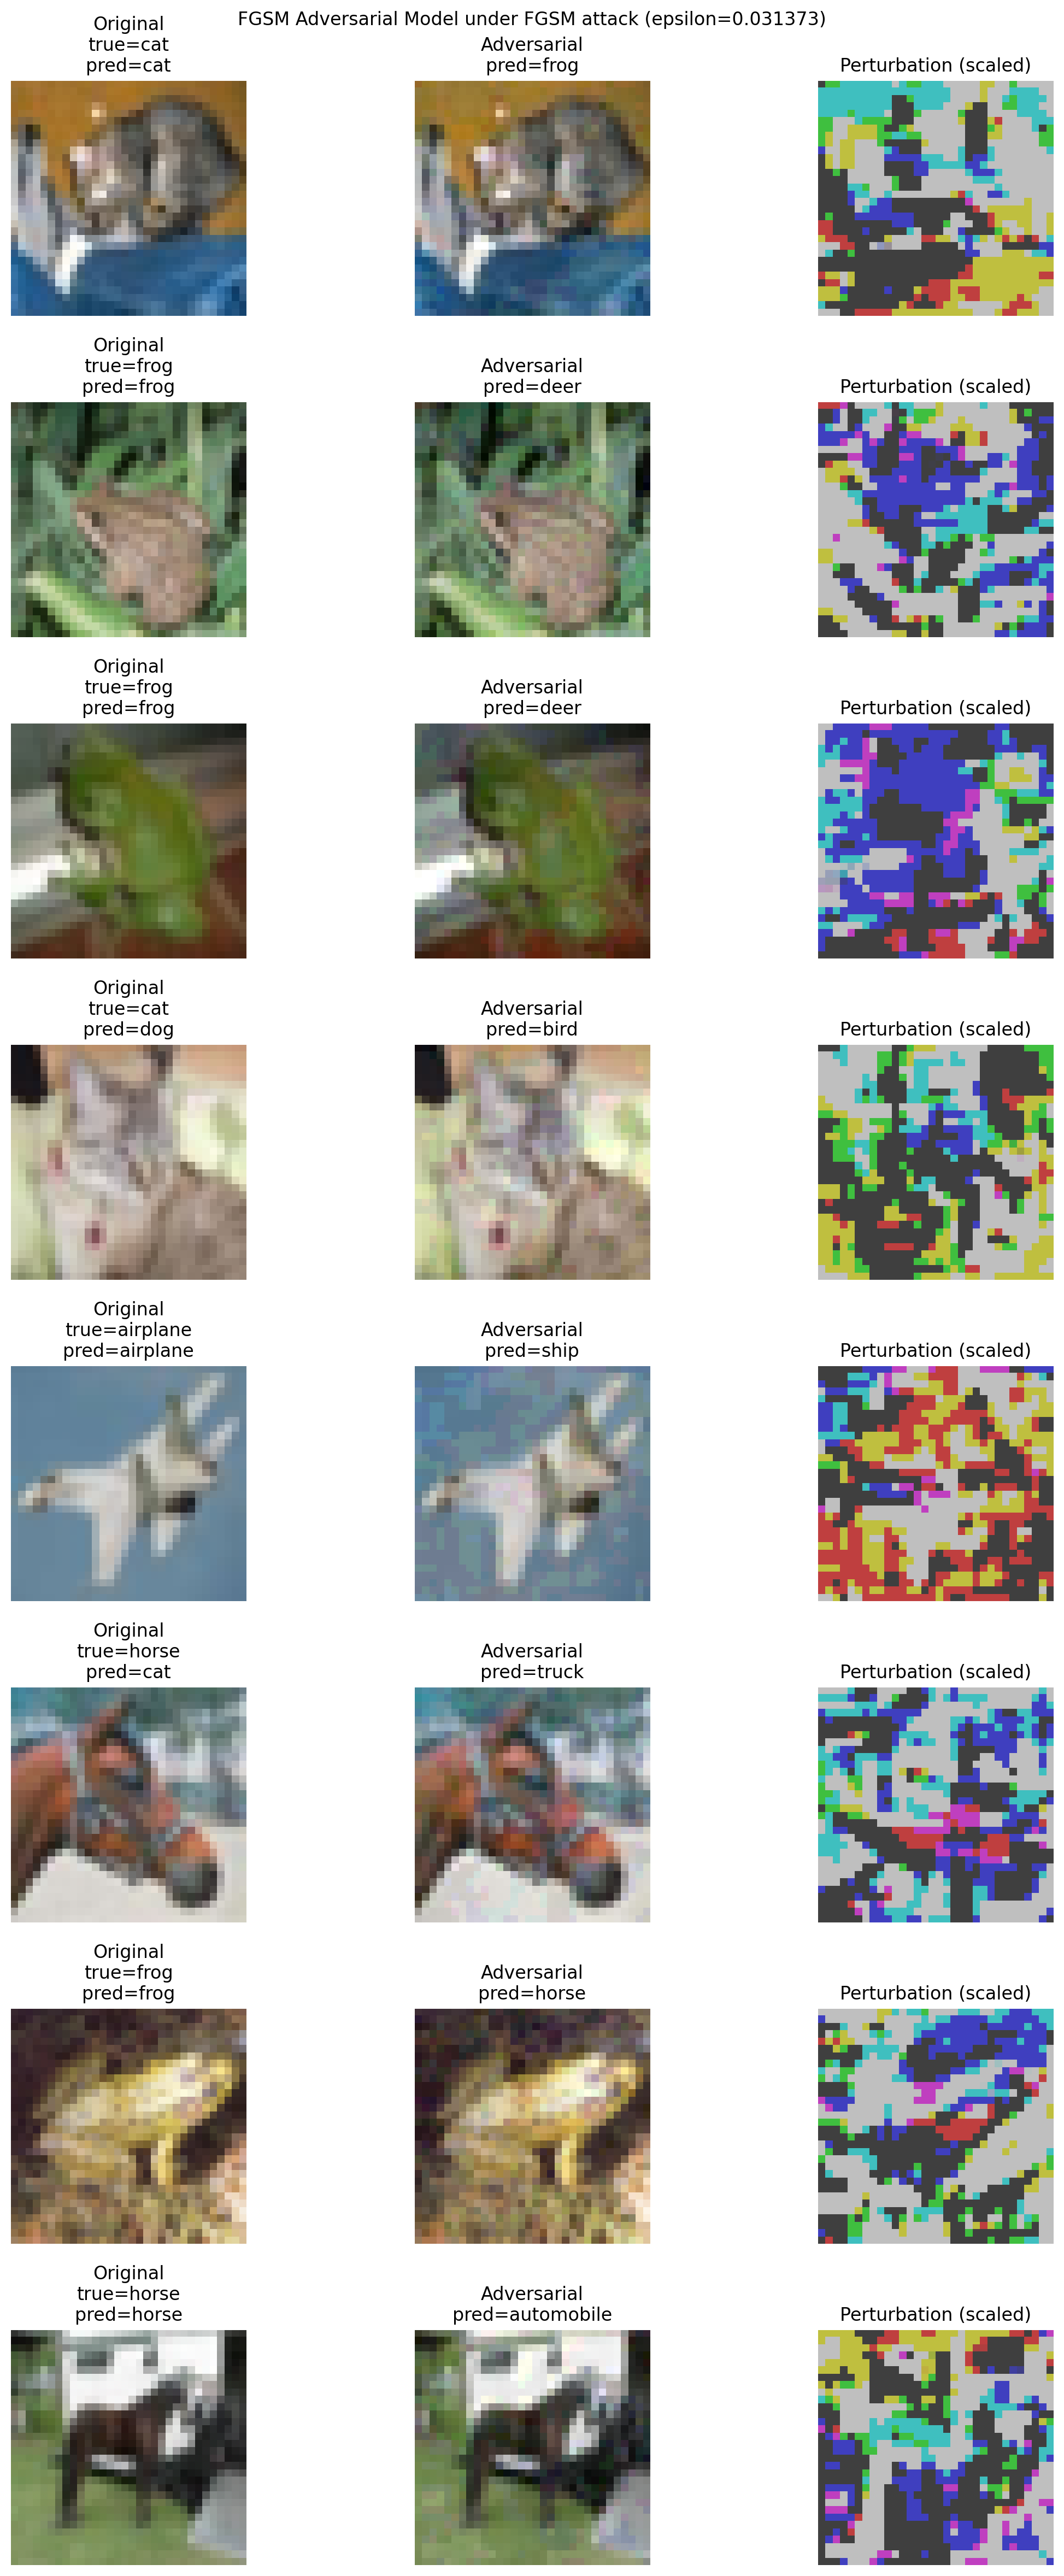
\includegraphics[width=0.49\linewidth]{../outputs/plots/attack_examples/fgsm_fgsm_eps_0.031373.png}
\hfill
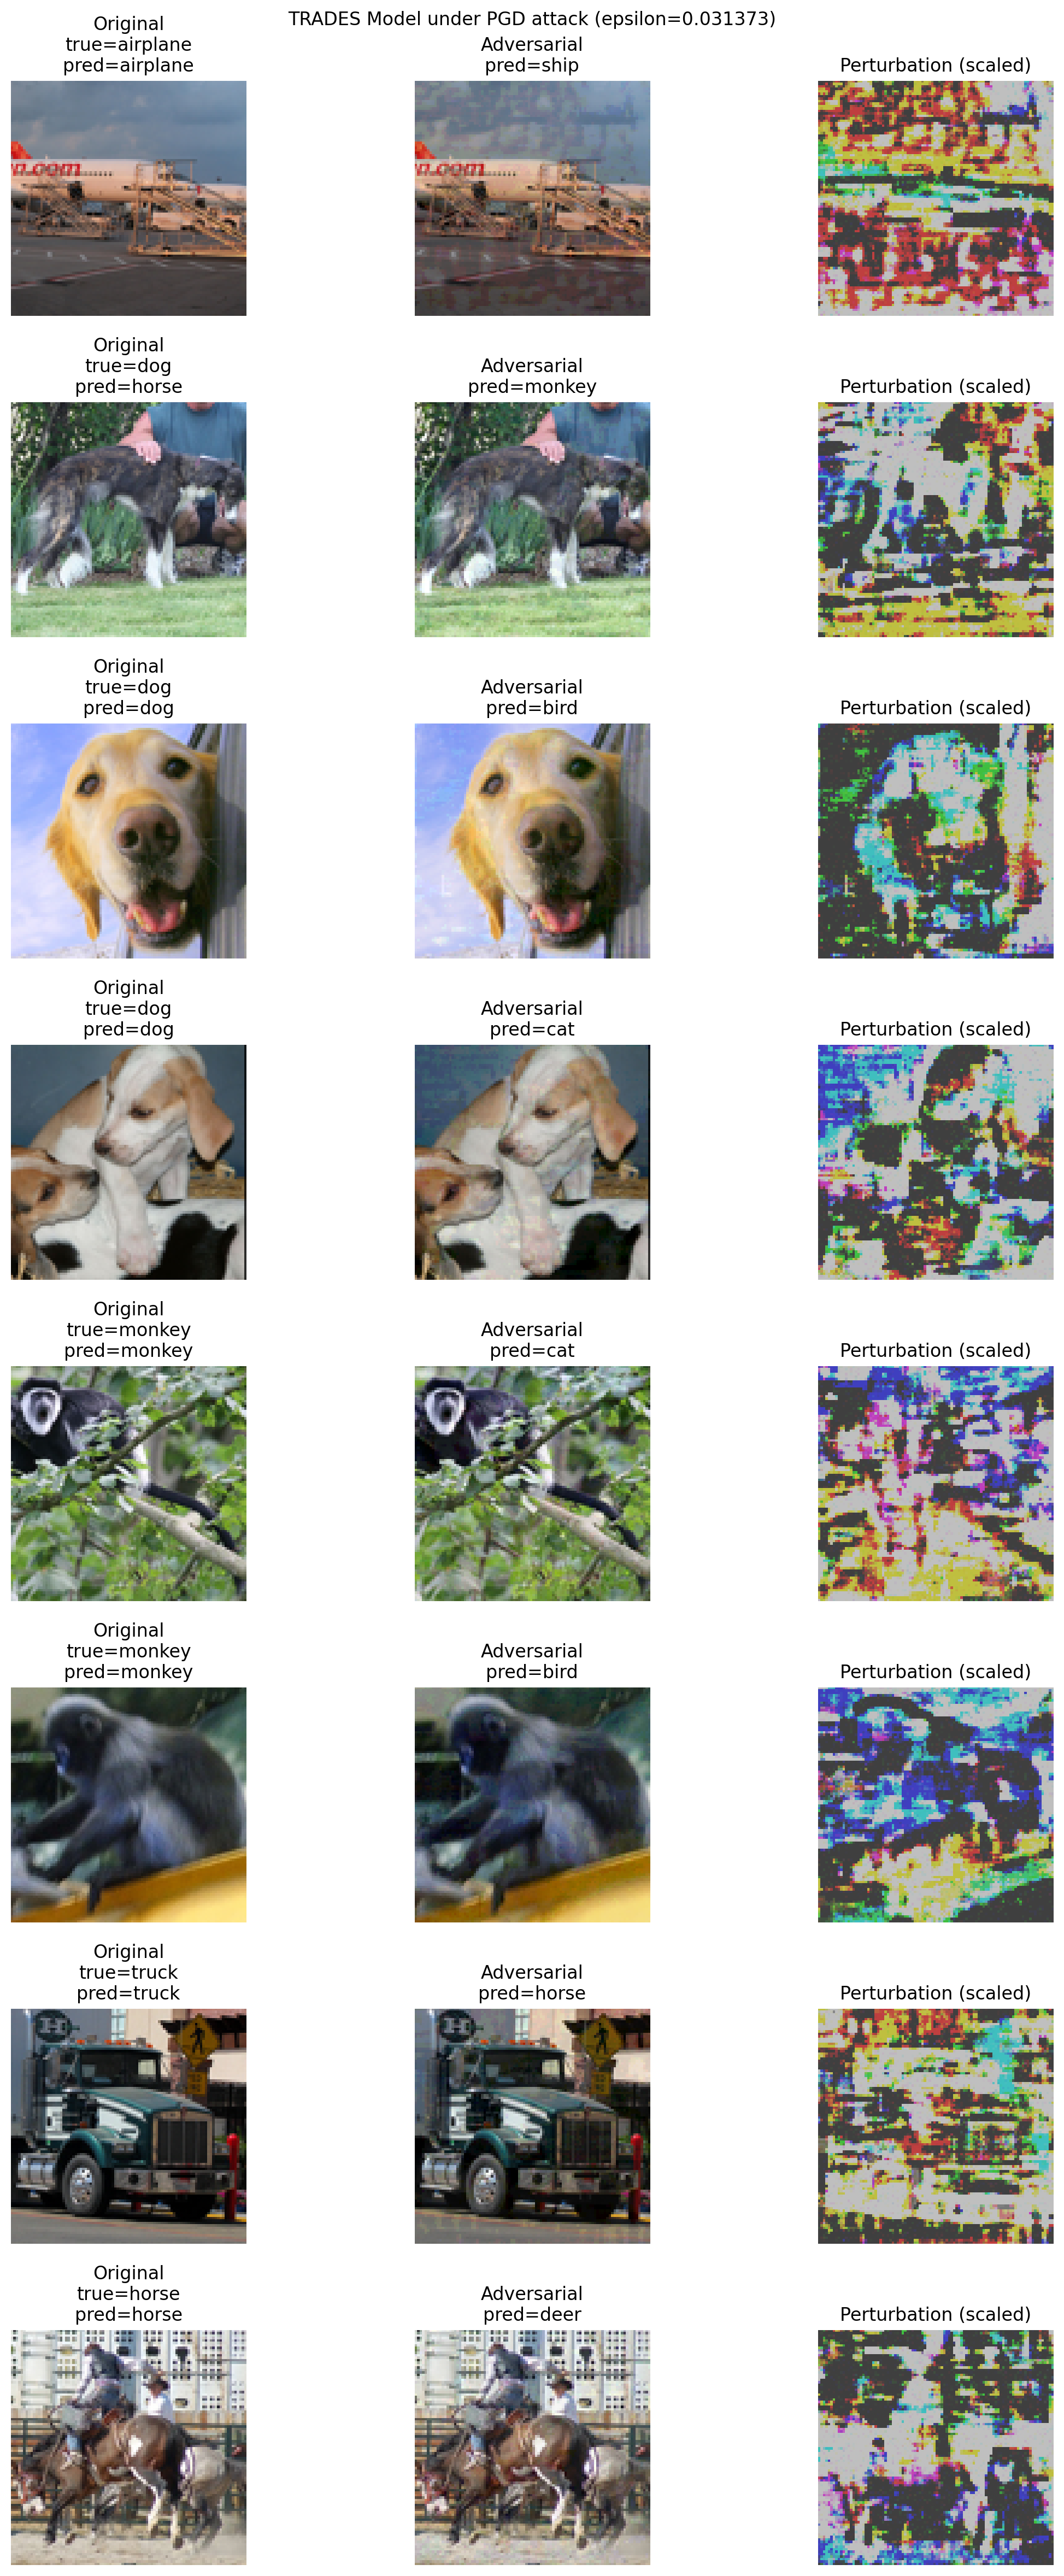
\includegraphics[width=0.49\linewidth]{../outputs/plots/attack_examples/trades_pgd_eps_0.031373.png}
\caption{FGSM-trained model under FGSM (left) and TRADES under PGD (right), $\epsilon=8/255$. Robust models still fail on some examples; panels match individual failures to the aggregate accuracies.}
\label{fig:attack-viz-fgsm-trades}
\end{figure}

\subsection{Resolution robustness}
\begin{figure}[t]
\centering
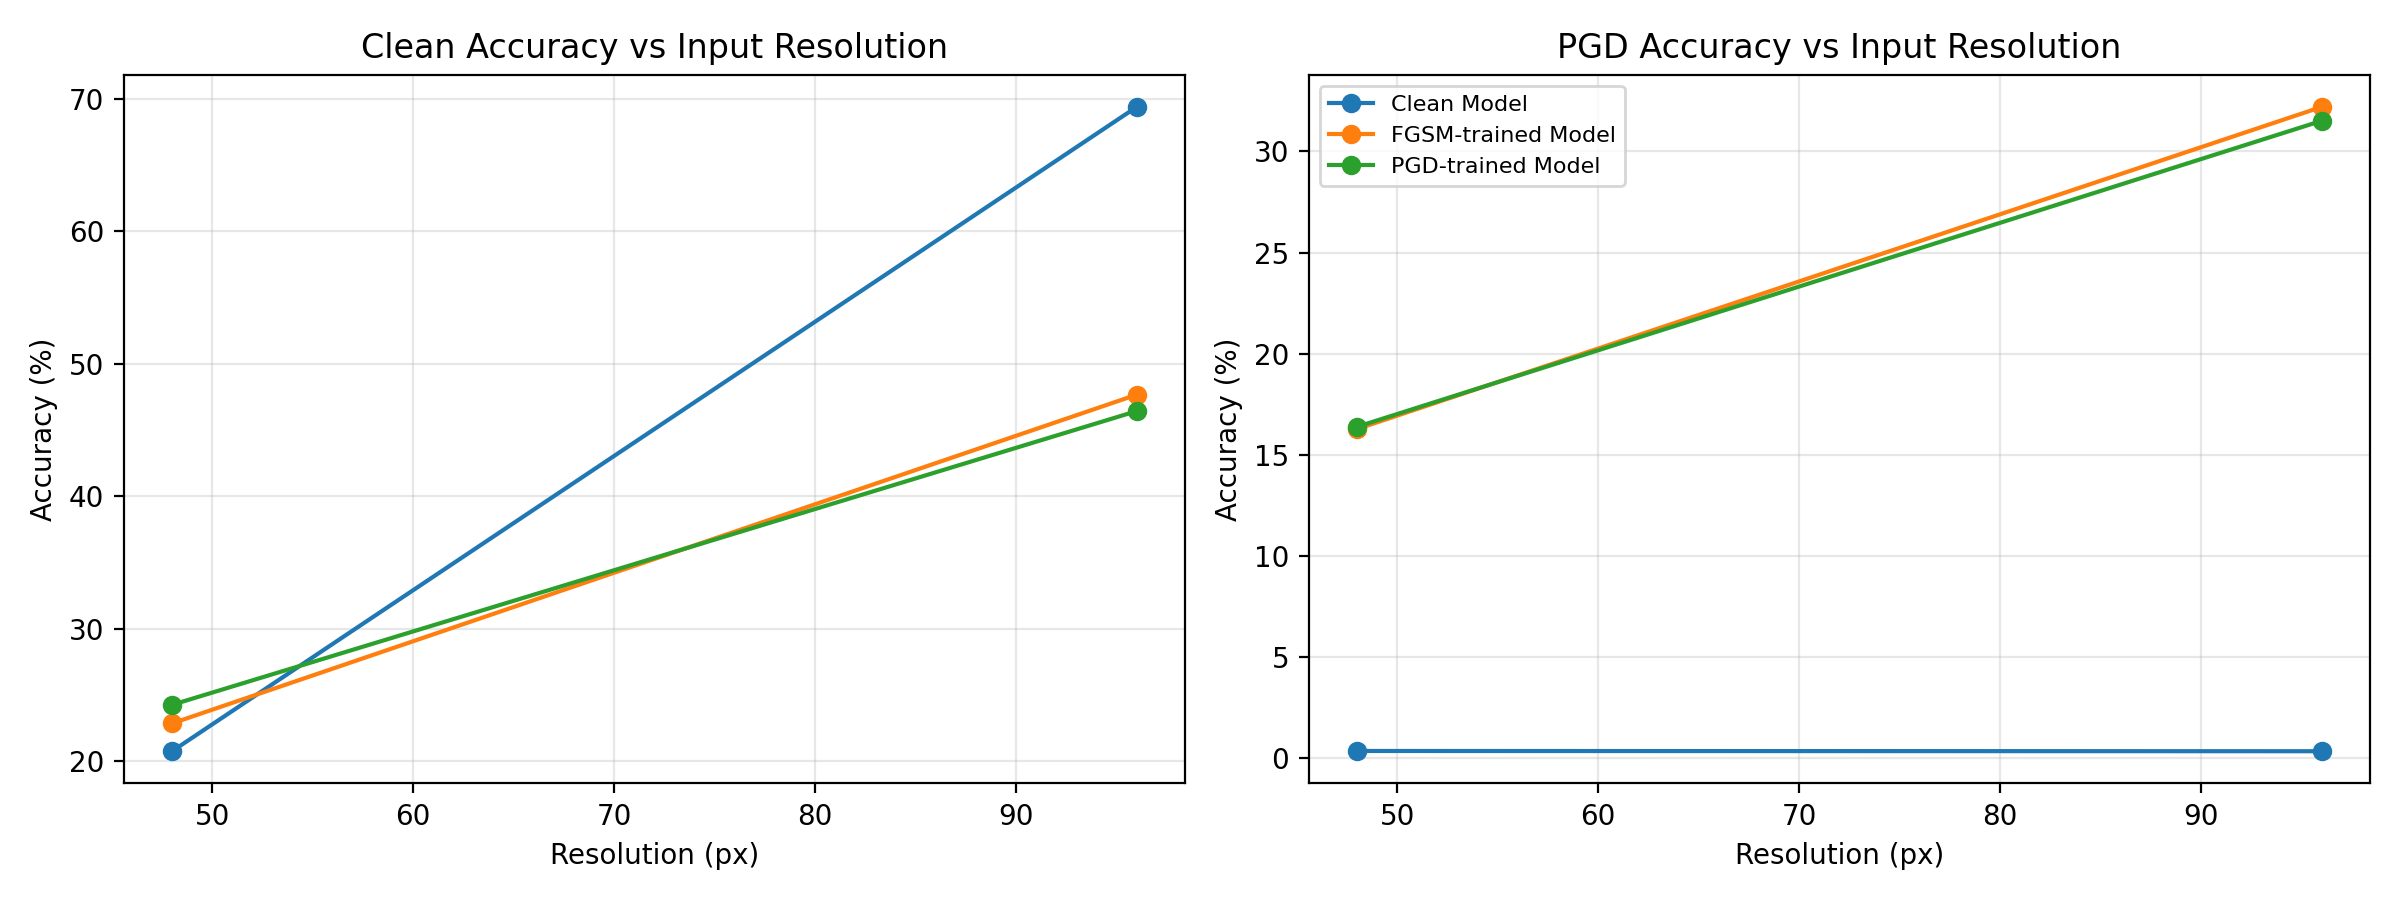
\includegraphics[width=\linewidth]{../outputs/plots/report/resolution_dual_plot_stl10.png}
\caption{Accuracy under resolution shift (96 to 48). Clean and adversarial performance both degrade, with robust models retaining significantly higher PGD accuracy than the clean model.}
\label{fig:resolution}
\end{figure}

When evaluated at lower resolution, all methods lose clean accuracy substantially. Still, robustly trained models maintain much better PGD performance than the clean model, indicating useful robustness under distribution shift.

\section{Limitations}
Robustness numbers here are conditional on the chosen attacks (FGSM/PGD with fixed step counts and step sizes) and on a single training run per method without seed ensembles. Stronger or adaptive attacks (e.g., more PGD restarts, AutoAttack-style pipelines) may reduce reported robust accuracy; that limitation is common and should be stated explicitly when interpreting defenses.

\section{Discussion}
Clean accuracy and adversarial accuracy trade off, consistent with prior work. Here PGD adversarial training wins on strong-PGD accuracy among the four setups; TRADES still offers a clear $\beta$ knob but needed more tuning here to match PGD.

\section{Conclusion}
STL-10 experiments with ResNet-18 compare clean, FGSM, PGD, and TRADES training under several $\ell_\infty$ budgets, plus transfer, per-class, resolution, and visualization checks. Robust training greatly improves PGD accuracy versus the clean baseline; numbers depend on the exact attack budget and training recipe. Code and outputs: \url{https://github.com/AshfakYeafi/CSE-850}.

Possible extensions: sweep TRADES $\beta\in\{1,3,6\}$, stronger PGD with restarts, repeat runs with different seeds.

\section{Declaration of individual contribution}
This project was completed individually by Ashfak Yeafi, including literature review, implementation, experiments, figures, and this manuscript.

\section*{References}
{\small
\begin{enumerate}
\item A. Madry, A. Makelov, L. Schmidt, D. Tsipras, and A. Vladu. Towards deep learning models resistant to adversarial attacks. In \textit{ICLR}, 2018.
\item H. Zhang, Y. Yu, J. Jiao, E. Xing, L. Ghaoui, and M. Jordan. Theoretically principled trade-off between robustness and accuracy. In \textit{ICML}, 2019.
\item I. Goodfellow, J. Shlens, and C. Szegedy. Explaining and harnessing adversarial examples. In \textit{ICLR}, 2015.
\end{enumerate}
}

\end{document}